\documentclass{ximera}

\begin{document}
	\author{Stitz-Zeager}
	\xmtitle{Exercises for Logarithmic Functions}{}

\mfpicnumber{1} \opengraphsfile{ExercisesforLogarithmicFunctions} % mfpic settings added 

\begin{question}
In Exercises \ref{rewritefirstex} - \ref{rewritelastex}, use the property: $b^{a} = c$ if and only if $\log_{b}(c) = a$ from Theorem \ref{logfcnprops} to rewrite the given equation in the other form.  That is, rewrite the exponential equations as logarithmic equations and rewrite the logarithmic equations as exponential equations.

\begin{problem}\label{rewritefirstex}
$2^{3} = 8$
\end{problem}

\begin{problem}
$5^{-3} = \frac{1}{125}$
\end{problem}

\begin{problem}
$4^{5/2} = 32$ 
\end{problem}

\begin{problem}
$\left(\frac{1}{3}\right)^{-2} = 9$ 
\end{problem}

\begin{problem}
$\left(\frac{4}{25}\right)^{-1/2} = \frac{5}{2}$  
\end{problem}

\begin{problem}
$10^{-3} = 0.001$ 
\end{problem}

\begin{problem}
$e^{0}  = 1$ 
\end{problem}

\begin{problem}
$\log_{5}(25) = 2$
\end{problem}

\begin{problem}
$\log_{25} (5) = \frac{1}{2}$
\end{problem}

\begin{problem}
$\log_{3} \left(\frac{1}{81} \right) = -4$
\end{problem}

\begin{problem}
$\log_{\frac{4}{3}} \left(\frac{3}{4} \right) = -1$ 
\end{problem}

\begin{problem}
$\log(100) = 2$ 
\end{problem}

\begin{problem}
$\log (0.1) = -1$
\end{problem}

\begin{problem}
$\ln(e) = 1$ 
\end{problem}

\begin{problem}\label{rewritelastex}
$\ln\left(\frac{1}{\sqrt{e}}\right) = -\frac{1}{2}$   
\end{problem}

\end{question}

\begin{question}
In Exercises \ref{simplifylogfirst} - \ref{simplifyloglast}, evaluate the expression without using a calculator.

\begin{problem}\label{simplifylogfirst}
$\log_{3} (27)$
\end{problem}

\begin{problem}
$\log_{6} (216)$
\end{problem}

\begin{problem}
$\log_{2} (32)$
\end{problem}

\begin{problem}
$\log_{6} \left( \frac{1}{36} \right)$
\end{problem}

\begin{problem}
$\log_{8} (4)$
\end{problem}

\begin{problem}
$\log_{36} (216)$
\end{problem}

\begin{problem}
$\log_{\frac{1}{5}} (625)$
\end{problem}

\begin{problem}
$\log_{\frac{1}{6}} (216)$
\end{problem}

\begin{problem}
$\log_{36} (36)$
\end{problem}

\begin{problem}
$\log \left(\frac{1}{1000000}\right)$
\end{problem}

\begin{problem}
$\log(0.01)$
\end{problem}

\begin{problem}
$\ln\left(e^3\right)$
\end{problem}

\begin{problem}
$\log_{4} (8)$
\end{problem}

\begin{problem}
$\log_{6} (1)$
\end{problem}

\begin{problem}
$\log_{13} \left(\sqrt{13}\right)$
\end{problem}

\begin{problem}
$\log_{36} \left(\sqrt[4]{36}\right)$
\end{problem}

\begin{problem}
$7^{\log_{7} (3)}$
\end{problem}

\begin{problem}
$36^{\log_{36}(216)}$
\end{problem}

\begin{problem}
$\log_{36} \left(36^{216}\right)$
\end{problem}

\begin{problem}
$\ln \left(e^{5} \right)$
\end{problem}

\begin{problem}
$\log \left(\sqrt[9]{10^{11}}\right)$
\end{problem}

\begin{problem}
$\log\left( \sqrt[3]{10^5} \right)$
\end{problem}

\begin{problem}
$\ln \left( \frac{1}{\sqrt{e}}\right)$
\end{problem}

\begin{problem}
$\log_{5} \left(3^{\log_{3} (5)}\right)$
\end{problem}

\begin{problem}
$\log\left(e^{\ln(100)}\right)$
\end{problem}

\begin{problem}
$\log_{2}\left(3^{-\log_{3}(2)}\right)$
\end{problem}

\begin{problem}\label{simplifyloglast}
$\ln\left(42^{6\log(1)}\right)$
\end{problem}
\end{question}

\begin{question}
In Exercises \ref{domainlogfirst} - \ref{domainloglast}, find the domain of the function.

\begin{problem}\label{domainlogfirst}
$f(x) = \ln(x^{2} + 1)$
\end{problem}

\begin{problem}
$f(x) = \log_{7}(4x + 8)$
\end{problem}

\begin{problem}
$g(t) = \ln(4t-20)$
\end{problem}

\begin{problem}
$g(t) = \log \left(t^2+9t+18\right)$
\end{problem}

\begin{problem}
$f(x) = \log \left(\dfrac{x + 2}{x^{2} - 1}\right)$
\end{problem}

\begin{problem}
$f(x) = \log\left(\dfrac{x^2+9x+18}{4x-20}\right)$
\end{problem}

\begin{problem}
$g(t) = \ln(7 - t) + \ln(t - 4)$
\end{problem}

\begin{problem}
$g(t) = \ln(4t-20) + \ln\left(t^2+9t+18\right)$
\end{problem}

\begin{problem}
$f(x) = \log\left(x^2+x+1\right)$
\end{problem}

\begin{problem}
$f(x) = \sqrt[4]{\log_{4} (x)}$
\end{problem}

\begin{problem}
$g(t) = \log_{9}(|t + 3| - 4)$
\end{problem}

\begin{problem}
$g(t) = \ln(\sqrt{t - 4} - 3)$
\end{problem}

\begin{problem}
$f(x) = \dfrac{1}{3 - \log_{5} (x)}$
\end{problem}

\begin{problem}
$f(x) = \dfrac{\sqrt{-1 - x}}{\log_{\frac{1}{2}} (x)}$
\end{problem}

\begin{problem}\label{domainloglast}
$f(x) = \ln(-2x^{3} - x^{2} + 13x - 6)$  
\end{problem}

\end{question}

\begin{question}
In Exercises \ref{graphlogfirst} - \ref{graphloglast}, sketch the graph of $g$ by starting with the graph of $f$ and using transformations.  Track at least three points of your choice and the vertical asymptote through the transformations. State the domain and range of $g$.

\begin{problem}\label{graphlogfirst}
$f(x) = \log_{2}(x)$, $g(x) = \log_{2}(x+1)$ 
\end{problem}

\begin{problem}
$f(x) = \log_{\frac{1}{3}}(x)$, $g(x) = \log_{\frac{1}{3}}(x)+1$
\end{problem}

\begin{problem}
$f(x) = \log_{3}(x)$, $g(x) = -\log_{3}(x-2)$
\end{problem}

\begin{problem}
$f(x) = \log(x)$, $g(x) = 2\log(x+20) -1$ 
\end{problem}

\begin{problem}
$f(t) = \log_{0.5}(t)$, $g(t) = 10 \log_{0.5}\left(\frac{t}{100}\right)$
\end{problem}

\begin{problem}
$f(t) = \log_{1.25}(t)$, $g(t) = \log_{1.25}(-t+1) + 2$
\end{problem}

\begin{problem}
$f(t) = \ln(t)$, $g(t) = -\ln(8-t)$
\end{problem}

\begin{problem}\label{graphloglast}
$f(t) = \ln(t)$, $g(t) = -10\ln\left(\frac{t}{10}\right)$ 
\end{problem}

\end{question}

\begin{problem}
Verify that each function in Exercises \ref{graphlogfirst} - \ref{graphloglast} is the inverse of the corresponding function in Exercises \ref{graphexpfirsta} - \ref{graphexplasta} in Section \ref{ExponentialFunctions}.  (Match up \#\ref{graphexpfirsta} and \#\ref{graphlogfirst}, and so on.)    
\end{problem}
  
\begin{question}
In Exercises, \ref{logformfirsta} - \ref{logformlasta}, the graph of a logarithmic function is given.  Find a formula for the function in the form $F(x) = a \cdot \log_{2}(bx-h)+k$.

\begin{problem}\label{logformfirsta} 
Points:  $\left( -\frac{5}{2}, -2 \right)$,  $\left(-2, -1 \right)$, $\left(-1,0 \right)$, \\
Asymptote:  $x = -3$. \\

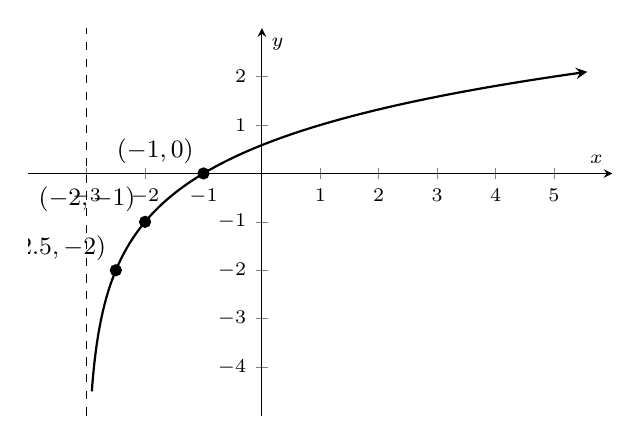
\begin{tikzpicture}
  \begin{axis}[
      axis lines=middle,
      xmin=-4, xmax=6,
      ymin=-5, ymax=3,
      xtick={-3,-2,-1,1,2,3,4,5},
      ytick={-4,-3,-2,-1,1,2},
      xlabel={$x$},
      ylabel={$y$},
      width=9cm,
      height=6.5cm,
      ticklabel style={font=\scriptsize},
      label style={font=\scriptsize},
    ]

    % Dashed vertical line
    \addplot[dashed, domain=-5:3] coordinates {(-3,-5) (-3,3)};

    % Parametric curve with arrows at both ends
    \addplot[
      thick,
      domain=-4.5:2.1,
      samples=200,
      ->,
      >=stealth
    ]
      ({2^(x+1)-3}, {x});

    % Points
    \addplot[only marks, mark=*] coordinates {
      (-2.5,-2)
      (-2,-1)
      (-1,0)
    };

    % Optional: label points if desired
    \node[font=\small, anchor=south east] at (axis cs:-2.5,-2) {$( -2.5, -2 )$};
    \node[font=\small, anchor=south east] at (axis cs:-2,-1) {$( -2, -1 )$};
    \node[font=\small, anchor=south east] at (axis cs:-1,0) {$( -1, 0 )$};

  \end{axis}
\end{tikzpicture}

\end{problem}

\begin{problem}
Points:  $\left( 1, -1 \right)$, $\left( 2, 0 \right)$, $\left(\frac{5}{2}, 1 \right)$ \\
Asymptote:  $x = 3$. \\

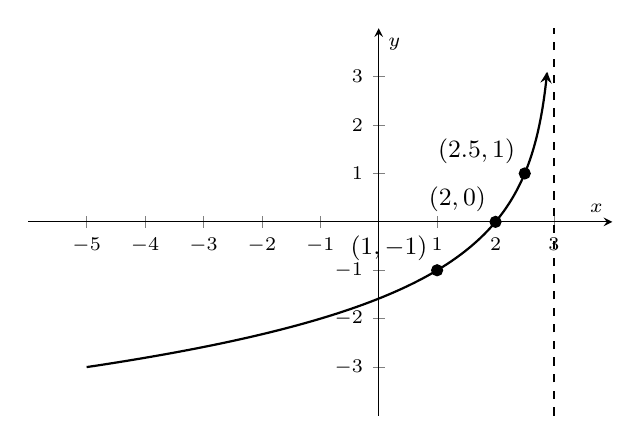
\begin{tikzpicture}
  \begin{axis}[
      axis lines=middle,
      xmin=-6, xmax=4,
      ymin=-4, ymax=4,
      xtick={-5,-4,-3,-2,-1,1,2,3},
      ytick={-3,-2,-1,1,2,3},
      xlabel={$x$},
      ylabel={$y$},
      width=9cm,
      height=6.5cm,
      ticklabel style={font=\scriptsize},
      label style={font=\scriptsize},
    ]

    % Dashed vertical asymptote at x = 3
    \addplot[dashed, domain=-4:4] coordinates {(3,-4) (3,4)};

    % Parametric curve with arrows at both ends
    \addplot[
      thick,
      domain=-3:3.1,
      samples=200,
      ->,
      >=stealth
    ]
      ({3 - 2^(-x)}, {x});

    % Points
    \addplot[only marks, mark=*] coordinates {
      (1,-1)
      (2,0)
      (2.5,1)
    };

    % Optional: label the points
    \node[font=\small, anchor=south east] at (axis cs:1,-1) {$(1,-1)$};
    \node[font=\small, anchor=south east] at (axis cs:2,0) {$(2,0)$};
    \node[font=\small, anchor=south east] at (axis cs:2.5,1) {$(2.5,1)$};

  \end{axis}
\end{tikzpicture}

\end{problem}

\begin{problem}
Points:  $\left(\frac{1}{2}, \frac{5}{2} \right)$, $\left(1, 3 \right)$, $\left(2, \frac{7}{2} \right)$, \\
Asymptote:  $x = 0$. \\

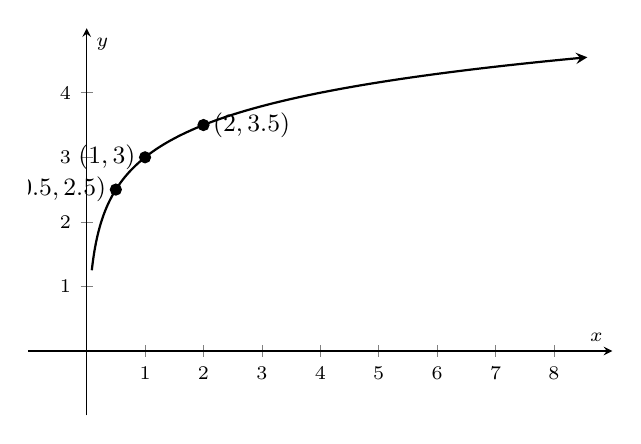
\begin{tikzpicture}
  \begin{axis}[
      axis lines=middle,
      xmin=-1, xmax=9,
      ymin=-1, ymax=5,
      xtick={1,2,3,4,5,6,7,8},
      ytick={1,2,3,4},
      xlabel={$x$},
      ylabel={$y$},
      width=9cm,
      height=6.5cm,
      ticklabel style={font=\scriptsize},
      label style={font=\scriptsize},
    ]

    % Parametric curve with arrows at both ends
    \addplot[
      thick,
      domain=1.25:4.55,
      samples=200,
      ->,
      >=stealth
    ]
      ({2^(2*x - 6)}, {x});

    % Points
    \addplot[only marks, mark=*] coordinates {
      (0.5,2.5)
      (1,3)
      (2,3.5)
    };

    % Optional point labels
    \node[font=\small, anchor=east] at (axis cs:0.5,2.5) {$(0.5, 2.5)$};
    \node[font=\small, anchor=east] at (axis cs:1,3) {$(1, 3)$};
    \node[font=\small, anchor=west] at (axis cs:2,3.5) {$(2, 3.5)$};

  \end{axis}
\end{tikzpicture}

\end{problem}

\begin{problem}\label{logformlasta} 
Points:  $\left( 6, -\frac{1}{2} \right)$, $\left(3,0 \right)$, $\left( \frac{3}{2}, \frac{1}{2} \right)$, \\
Asymptote:  $x = 0$.   \\

\begin{tikzpicture}
  \begin{axis}[
      axis lines=middle,
      xmin=-1, xmax=9,
      ymin=-4, ymax=4,
      xtick={1,2,3,7,8},
      ytick={-3,-2,-1,1,2,3},
      xlabel={$x$},
      ylabel={$y$},
      width=9cm,
      height=6.5cm,
      ticklabel style={font=\scriptsize},
      label style={font=\scriptsize},
    ]

    % Parametric curve: (3*(2^(-2t)), t)
    \addplot[
      thick,
      domain=-0.79:2,
      samples=200,
      ->,
      >=stealth
    ]
      ({3*(2^(-2*x))}, {x});

    % Points
    \addplot[only marks, mark=*] coordinates {
      (6,-0.5)
      (3,0)
      (1.5,0.5)
    };

    % Optional point labels
    \node[font=\small, anchor=west] at (axis cs:6,-0.5) {$(6,-0.5)$};
    \node[font=\small, anchor=west] at (axis cs:3,0) {$(3,0)$};
    \node[font=\small, anchor=west] at (axis cs:1.5,0.5) {$(1.5,0.5)$};

  \end{axis}
\end{tikzpicture}

\end{problem}
\end{question}

\begin{problem}\label{logformbase4exercise} 
Find a formula for each graph in Exercises \ref{logformfirsta} - \ref{logformlasta} of the form $G(x) =  a \cdot \log_{4}(bx-h)+k$.
\end{problem}

\begin{question}
In Exercises \ref{inverselogexpfirst} - \ref{inverselogexplast},  find the inverse of the function from the `procedural perspective' discussed in Example \ref{proceduralinverse} and graph the function and its inverse on the same set of axes.

\begin{problem}\label{inverselogexpfirst}
$f(x) = 3^{x + 2} - 4$
\end{problem}

\begin{problem}
$f(x) = \log_{4}(x - 1)$
\end{problem}

\begin{problem}
$g(t)= -2^{-t} + 1$
\end{problem}

\begin{problem}\label{inverselogexplast}
$g(t) = 5\log(t) - 2$ 
\end{problem}

\end{question}
\begin{question}
In Exercises \ref{decomposebasiclogfirst} - \ref{decomposebasicloglast}, write the given function as a nontrivial decomposition of functions as directed.

\begin{problem}\label{decomposebasiclogfirst}
For $f(x) = \log_{2}(x+3) + 4$, find functions $g$ and $h$ so that $f=g+h$. 
\end{problem}

\begin{problem}
For $f(x) = \log(2x) - e^{-x}$, find functions $g$ and $h$ so that $f=g-h$. 
\end{problem}

\begin{problem}
For $f(t) = 3t \log(t)$, find functions $g$ and $h$ so that $f=gh$.
\end{problem}

\begin{problem}
For $r(x) = \dfrac{\ln(x)}{x}$, find functions $f$ and $g$ so $r = \dfrac{f}{g}$.
\end{problem}

\begin{problem}
For $k(t) = \ln(t^2+1)$, find functions $f$ and $g$  so that $k = g \circ f$.
\end{problem}

\begin{problem}\label{decomposebasicloglast}
For $p(z) = (\ln(z))^2$, find functions $f$ and $g$ so $p = g \circ f$. 
\end{problem}
\end{question}

\begin{question}\label{logarithmicscales}
(Logarithmic Scales) In Exercises \ref{Richterexercise} - \ref{pHexercise}, we introduce three widely used measurement scales which involve common logarithms: the Richter scale, the decibel scale and the pH scale.  The computations involved in all three scales are nearly identical so pay attention to the subtle differences.

\begin{problem}\label{Richterexercise} 
Earthquakes are complicated events and it is not our intent to provide a complete discussion of the science involved in them.  Instead, we refer the interested reader to a solid course in Geology\footnote{Rock-solid, perhaps?} or the U.S. Geological Survey's Earthquake Hazards Program found \href{http://earthquake.usgs.gov/}{\underline{here}} and present only a simplified version of the \href{http://en.wikipedia.org/wiki/Richter_scale}{\underline{Richter scale}}.  The Richter scale measures the magnitude of an earthquake by comparing the amplitude of the seismic waves of the given earthquake to those of a ``magnitude 0 event'', which was chosen to be a seismograph reading of $0.001$ millimeters recorded on a seismometer 100 kilometers from the earthquake's epicenter.  Specifically, the magnitude of an earthquake is given by \[M(x) = \log \left(\dfrac{x}{0.001}\right)\] where $x$ is the seismograph reading in millimeters of the earthquake recorded 100 kilometers from the epicenter.  

\begin{enumerate}

\item Show that $M(0.001) = 0$.
\item Compute $M(80,000)$.
\item Show that an earthquake which registered 6.7 on the Richter scale had a seismograph reading ten times larger than one which measured 5.7.
\item Find two news stories about recent earthquakes which give their magnitudes on the Richter scale.  How many times larger was the seismograph reading of the earthquake with larger magnitude?

\end{enumerate}

\end{problem}

\begin{problem}\label{decibelexercise}
While the decibel scale can be used in many disciplines,\footnote{See this  \href{http://en.wikipedia.org/wiki/Decibel}{\underline{webpage}} for more information.} we shall restrict our attention to its use in acoustics, specifically its use in measuring the intensity level of sound. The Sound Intensity Level $L$ (measured in decibels) of a sound intensity $I$ (measured in watts per square meter) is given by \[L(I) = 10\log\left( \dfrac{I}{10^{-12}} \right).\] Like the Richter scale, this scale compares $I$ to baseline: $10^{-12} \frac{W}{m^{2}}$ is the threshold of human hearing. 

\begin{enumerate}

\item Compute $L(10^{-6})$.
\item Damage to your hearing can start with short term exposure to sound levels around 115 decibels.  What intensity $I$ is needed to produce this level? 
\item Compute $L(1)$.  How does this compare with the threshold of pain which is around 140 decibels?

\end{enumerate}
\end{problem}

\begin{problem}\label{pHexercise}
The pH of a solution is a measure of its acidity or alkalinity.  Specifically, $\mbox{pH} = -\log[\mbox{H}^{+}]$ where $[\mbox{H}^{+}]$ is the hydrogen ion concentration in moles per liter.  A solution with a pH less than 7 is an acid, one with a pH greater than 7 is a base (alkaline) and a pH of 7 is regarded as neutral.

\begin{enumerate}

\item The hydrogen ion concentration of pure water is $[\mbox{H}^{+}] = 10^{-7}$.  Find its pH.
\item Find the pH of a solution with $[\mbox{H}^{+}] = 6.3 \times 10^{-13}$.
\item The pH of gastric acid (the acid in your stomach) is about $0.7$.  What is the corresponding hydrogen ion concentration?

\end{enumerate}

\end{problem}

\end{question}

\begin{problem}
Use the definition of logarithm to explain why  $\log_{b} 1 = 0$ and $\log_{b} b = 1$ for every $b > 0, \; b \neq 1$.
\end{problem}

\end{document}
